% Options for packages loaded elsewhere
\PassOptionsToPackage{unicode}{hyperref}
\PassOptionsToPackage{hyphens}{url}
%
\documentclass[
]{article}
\usepackage{amsmath,amssymb}
\usepackage{iftex}
\ifPDFTeX
  \usepackage[T1]{fontenc}
  \usepackage[utf8]{inputenc}
  \usepackage{textcomp} % provide euro and other symbols
\else % if luatex or xetex
  \usepackage{unicode-math} % this also loads fontspec
  \defaultfontfeatures{Scale=MatchLowercase}
  \defaultfontfeatures[\rmfamily]{Ligatures=TeX,Scale=1}
\fi
\usepackage{lmodern}
\ifPDFTeX\else
  % xetex/luatex font selection
\fi
% Use upquote if available, for straight quotes in verbatim environments
\IfFileExists{upquote.sty}{\usepackage{upquote}}{}
\IfFileExists{microtype.sty}{% use microtype if available
  \usepackage[]{microtype}
  \UseMicrotypeSet[protrusion]{basicmath} % disable protrusion for tt fonts
}{}
\makeatletter
\@ifundefined{KOMAClassName}{% if non-KOMA class
  \IfFileExists{parskip.sty}{%
    \usepackage{parskip}
  }{% else
    \setlength{\parindent}{0pt}
    \setlength{\parskip}{6pt plus 2pt minus 1pt}}
}{% if KOMA class
  \KOMAoptions{parskip=half}}
\makeatother
\usepackage{xcolor}
\usepackage[margin=1in]{geometry}
\usepackage{color}
\usepackage{fancyvrb}
\newcommand{\VerbBar}{|}
\newcommand{\VERB}{\Verb[commandchars=\\\{\}]}
\DefineVerbatimEnvironment{Highlighting}{Verbatim}{commandchars=\\\{\}}
% Add ',fontsize=\small' for more characters per line
\usepackage{framed}
\definecolor{shadecolor}{RGB}{248,248,248}
\newenvironment{Shaded}{\begin{snugshade}}{\end{snugshade}}
\newcommand{\AlertTok}[1]{\textcolor[rgb]{0.94,0.16,0.16}{#1}}
\newcommand{\AnnotationTok}[1]{\textcolor[rgb]{0.56,0.35,0.01}{\textbf{\textit{#1}}}}
\newcommand{\AttributeTok}[1]{\textcolor[rgb]{0.13,0.29,0.53}{#1}}
\newcommand{\BaseNTok}[1]{\textcolor[rgb]{0.00,0.00,0.81}{#1}}
\newcommand{\BuiltInTok}[1]{#1}
\newcommand{\CharTok}[1]{\textcolor[rgb]{0.31,0.60,0.02}{#1}}
\newcommand{\CommentTok}[1]{\textcolor[rgb]{0.56,0.35,0.01}{\textit{#1}}}
\newcommand{\CommentVarTok}[1]{\textcolor[rgb]{0.56,0.35,0.01}{\textbf{\textit{#1}}}}
\newcommand{\ConstantTok}[1]{\textcolor[rgb]{0.56,0.35,0.01}{#1}}
\newcommand{\ControlFlowTok}[1]{\textcolor[rgb]{0.13,0.29,0.53}{\textbf{#1}}}
\newcommand{\DataTypeTok}[1]{\textcolor[rgb]{0.13,0.29,0.53}{#1}}
\newcommand{\DecValTok}[1]{\textcolor[rgb]{0.00,0.00,0.81}{#1}}
\newcommand{\DocumentationTok}[1]{\textcolor[rgb]{0.56,0.35,0.01}{\textbf{\textit{#1}}}}
\newcommand{\ErrorTok}[1]{\textcolor[rgb]{0.64,0.00,0.00}{\textbf{#1}}}
\newcommand{\ExtensionTok}[1]{#1}
\newcommand{\FloatTok}[1]{\textcolor[rgb]{0.00,0.00,0.81}{#1}}
\newcommand{\FunctionTok}[1]{\textcolor[rgb]{0.13,0.29,0.53}{\textbf{#1}}}
\newcommand{\ImportTok}[1]{#1}
\newcommand{\InformationTok}[1]{\textcolor[rgb]{0.56,0.35,0.01}{\textbf{\textit{#1}}}}
\newcommand{\KeywordTok}[1]{\textcolor[rgb]{0.13,0.29,0.53}{\textbf{#1}}}
\newcommand{\NormalTok}[1]{#1}
\newcommand{\OperatorTok}[1]{\textcolor[rgb]{0.81,0.36,0.00}{\textbf{#1}}}
\newcommand{\OtherTok}[1]{\textcolor[rgb]{0.56,0.35,0.01}{#1}}
\newcommand{\PreprocessorTok}[1]{\textcolor[rgb]{0.56,0.35,0.01}{\textit{#1}}}
\newcommand{\RegionMarkerTok}[1]{#1}
\newcommand{\SpecialCharTok}[1]{\textcolor[rgb]{0.81,0.36,0.00}{\textbf{#1}}}
\newcommand{\SpecialStringTok}[1]{\textcolor[rgb]{0.31,0.60,0.02}{#1}}
\newcommand{\StringTok}[1]{\textcolor[rgb]{0.31,0.60,0.02}{#1}}
\newcommand{\VariableTok}[1]{\textcolor[rgb]{0.00,0.00,0.00}{#1}}
\newcommand{\VerbatimStringTok}[1]{\textcolor[rgb]{0.31,0.60,0.02}{#1}}
\newcommand{\WarningTok}[1]{\textcolor[rgb]{0.56,0.35,0.01}{\textbf{\textit{#1}}}}
\usepackage{graphicx}
\makeatletter
\newsavebox\pandoc@box
\newcommand*\pandocbounded[1]{% scales image to fit in text height/width
  \sbox\pandoc@box{#1}%
  \Gscale@div\@tempa{\textheight}{\dimexpr\ht\pandoc@box+\dp\pandoc@box\relax}%
  \Gscale@div\@tempb{\linewidth}{\wd\pandoc@box}%
  \ifdim\@tempb\p@<\@tempa\p@\let\@tempa\@tempb\fi% select the smaller of both
  \ifdim\@tempa\p@<\p@\scalebox{\@tempa}{\usebox\pandoc@box}%
  \else\usebox{\pandoc@box}%
  \fi%
}
% Set default figure placement to htbp
\def\fps@figure{htbp}
\makeatother
\setlength{\emergencystretch}{3em} % prevent overfull lines
\providecommand{\tightlist}{%
  \setlength{\itemsep}{0pt}\setlength{\parskip}{0pt}}
\setcounter{secnumdepth}{-\maxdimen} % remove section numbering
\usepackage{ctex}
\usepackage{bookmark}
\IfFileExists{xurl.sty}{\usepackage{xurl}}{} % add URL line breaks if available
\urlstyle{same}
\hypersetup{
  pdftitle={homework2},
  pdfauthor={zza},
  hidelinks,
  pdfcreator={LaTeX via pandoc}}

\title{homework2}
\author{zza}
\date{2025-06-29}

\begin{document}
\maketitle

\subsection{1 Lodinng and cleaning}\label{lodinng-and-cleaning}

\subsubsection{a}\label{a}

\begin{Shaded}
\begin{Highlighting}[]
\NormalTok{ca\_pa }\OtherTok{\textless{}{-}} \FunctionTok{read.csv}\NormalTok{(}\StringTok{"calif\_penn\_2011.csv"}\NormalTok{, }\AttributeTok{stringsAsFactors =} \ConstantTok{FALSE}\NormalTok{)}
\end{Highlighting}
\end{Shaded}

\subsubsection{b}\label{b}

\begin{verbatim}
## 行数: 11275
\end{verbatim}

\begin{verbatim}
## 列数: 34
\end{verbatim}

\subsubsection{c}\label{c}

\begin{Shaded}
\begin{Highlighting}[]
\NormalTok{temp}\OtherTok{\textless{}{-}}\FunctionTok{colSums}\NormalTok{(}\FunctionTok{apply}\NormalTok{(ca\_pa,}\FunctionTok{c}\NormalTok{(}\DecValTok{1}\NormalTok{,}\DecValTok{2}\NormalTok{),is.na))}
\end{Highlighting}
\end{Shaded}

对ca\_pa里的所有元素进行is.na判断,并对apply返回的逻辑值矩阵进行按列求和,得出每一列缺失值的数目

\subsubsection{d}\label{d}

\begin{Shaded}
\begin{Highlighting}[]
\NormalTok{  ca\_pa\_clean}\OtherTok{\textless{}{-}}\FunctionTok{na.omit}\NormalTok{(ca\_pa) }\DocumentationTok{\#\#清除后的dataframe}
\end{Highlighting}
\end{Shaded}

\subsubsection{e}\label{e}

\begin{verbatim}
## 清除的行数: 670
\end{verbatim}

\subsubsection{f}\label{f}

\begin{verbatim}
## c中各列na数量的总和: 3034
\end{verbatim}

其中c中的结果和大于清除的总行数,这正说明了它们的一致性,因为每行可能含有多个na值

\subsection{2 This very new House}\label{this-very-new-house}

\subsubsection{a. 绘制房价中位数与 Built\_2005\_or\_later
的关系图}\label{a.-ux7ed8ux5236ux623fux4ef7ux4e2dux4f4dux6570ux4e0e-built_2005_or_later-ux7684ux5173ux7cfbux56fe}

\begin{Shaded}
\begin{Highlighting}[]
\CommentTok{\# 绘制散点图,房价中位数列是 Median\_house\_value,Built\_2005\_or\_later 是对应列}
\FunctionTok{plot}\NormalTok{(}
  \AttributeTok{x =}\NormalTok{ ca\_pa\_clean}\SpecialCharTok{$}\NormalTok{Built\_2005\_or\_later, }
  \AttributeTok{y =}\NormalTok{ ca\_pa\_clean}\SpecialCharTok{$}\NormalTok{Median\_house\_value,}
  \AttributeTok{main =} \StringTok{"Median House Prices vs Built\_2005\_or\_later"}\NormalTok{,}
  \AttributeTok{xlab =} \StringTok{"Percentage of Houses Built 2005 or Later"}\NormalTok{,}
  \AttributeTok{ylab =} \StringTok{"Median House Price"}\NormalTok{,}
  \AttributeTok{pch =} \DecValTok{16}\NormalTok{, }
  \AttributeTok{col =} \StringTok{"steelblue"}  
\NormalTok{)}

\FunctionTok{abline}\NormalTok{(}\FunctionTok{lm}\NormalTok{(Median\_house\_value }\SpecialCharTok{\textasciitilde{}}\NormalTok{ Built\_2005\_or\_later, }\AttributeTok{data =}\NormalTok{ ca\_pa\_clean), }
       \AttributeTok{col =} \StringTok{"red"}\NormalTok{, }
       \AttributeTok{lwd =} \DecValTok{2}\NormalTok{)  }
\end{Highlighting}
\end{Shaded}

\pandocbounded{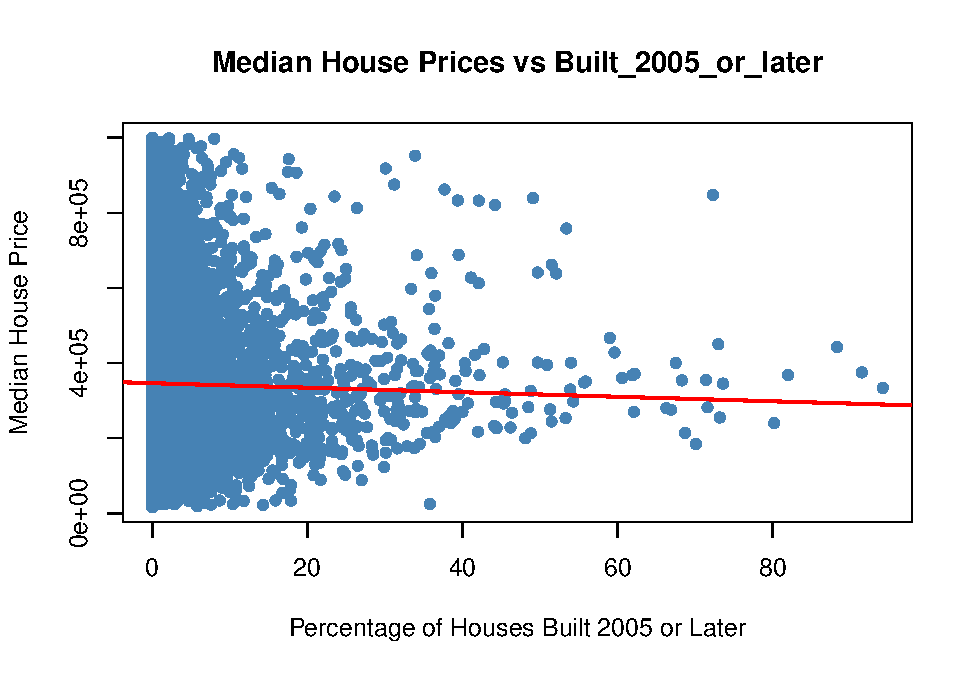
\includegraphics[keepaspectratio]{homework2_files/figure-latex/unnamed-chunk-7-1.pdf}}

\subsubsection{b}\label{b-1}

\begin{Shaded}
\begin{Highlighting}[]
\CommentTok{\# 筛选加利福尼亚州(STATEFP == 6)和宾夕法尼亚州(STATEFP == 42)的数据}
\NormalTok{ca\_data }\OtherTok{\textless{}{-}}\NormalTok{ ca\_pa\_clean[ca\_pa\_clean}\SpecialCharTok{$}\NormalTok{STATEFP }\SpecialCharTok{==} \DecValTok{6}\NormalTok{, ]}
\NormalTok{pa\_data }\OtherTok{\textless{}{-}}\NormalTok{ ca\_pa\_clean[ca\_pa\_clean}\SpecialCharTok{$}\NormalTok{STATEFP }\SpecialCharTok{==} \DecValTok{42}\NormalTok{, ]}

\CommentTok{\# 绘制分组散点图,使用 par(mfrow = c(1, 2)) 将图形排列在一行两列}
\FunctionTok{par}\NormalTok{(}\AttributeTok{mfrow =} \FunctionTok{c}\NormalTok{(}\DecValTok{1}\NormalTok{, }\DecValTok{2}\NormalTok{))  }

\CommentTok{\# 加利福尼亚州的散点图}
\FunctionTok{plot}\NormalTok{(}
  \AttributeTok{x =}\NormalTok{ ca\_data}\SpecialCharTok{$}\NormalTok{Built\_2005\_or\_later, }
  \AttributeTok{y =}\NormalTok{ ca\_data}\SpecialCharTok{$}\NormalTok{Median\_house\_value,}
  \AttributeTok{main =} \StringTok{"California:"}\NormalTok{,}
  \AttributeTok{xlab =} \StringTok{"Percentage of Houses Built 2005 or Later"}\NormalTok{,}
  \AttributeTok{ylab =} \StringTok{"Median House Price"}\NormalTok{,}
  \AttributeTok{pch =} \DecValTok{16}\NormalTok{,}
  \AttributeTok{col =} \StringTok{"forestgreen"}
\NormalTok{)}
\FunctionTok{abline}\NormalTok{(}\FunctionTok{lm}\NormalTok{(Median\_house\_value }\SpecialCharTok{\textasciitilde{}}\NormalTok{ Built\_2005\_or\_later, }\AttributeTok{data =}\NormalTok{ ca\_data), }
       \AttributeTok{col =} \StringTok{"red"}\NormalTok{, }
       \AttributeTok{lwd =} \DecValTok{2}\NormalTok{)}

\CommentTok{\# 宾夕法尼亚州的散点图}
\FunctionTok{plot}\NormalTok{(}
  \AttributeTok{x =}\NormalTok{ pa\_data}\SpecialCharTok{$}\NormalTok{Built\_2005\_or\_later, }
  \AttributeTok{y =}\NormalTok{ pa\_data}\SpecialCharTok{$}\NormalTok{Median\_house\_value,}
  \AttributeTok{main =} \StringTok{"Pennsylvania: "}\NormalTok{,}
  \AttributeTok{xlab =} \StringTok{"Percentage of Houses Built 2005 or Later"}\NormalTok{,}
  \AttributeTok{ylab =} \StringTok{"Median House Price"}\NormalTok{,}
  \AttributeTok{pch =} \DecValTok{16}\NormalTok{,}
  \AttributeTok{col =} \StringTok{"orange"}
\NormalTok{)}
\FunctionTok{abline}\NormalTok{(}\FunctionTok{lm}\NormalTok{(Median\_house\_value }\SpecialCharTok{\textasciitilde{}}\NormalTok{ Built\_2005\_or\_later, }\AttributeTok{data =}\NormalTok{ pa\_data), }
       \AttributeTok{col =} \StringTok{"red"}\NormalTok{, }
       \AttributeTok{lwd =} \DecValTok{2}\NormalTok{)}
\end{Highlighting}
\end{Shaded}

\pandocbounded{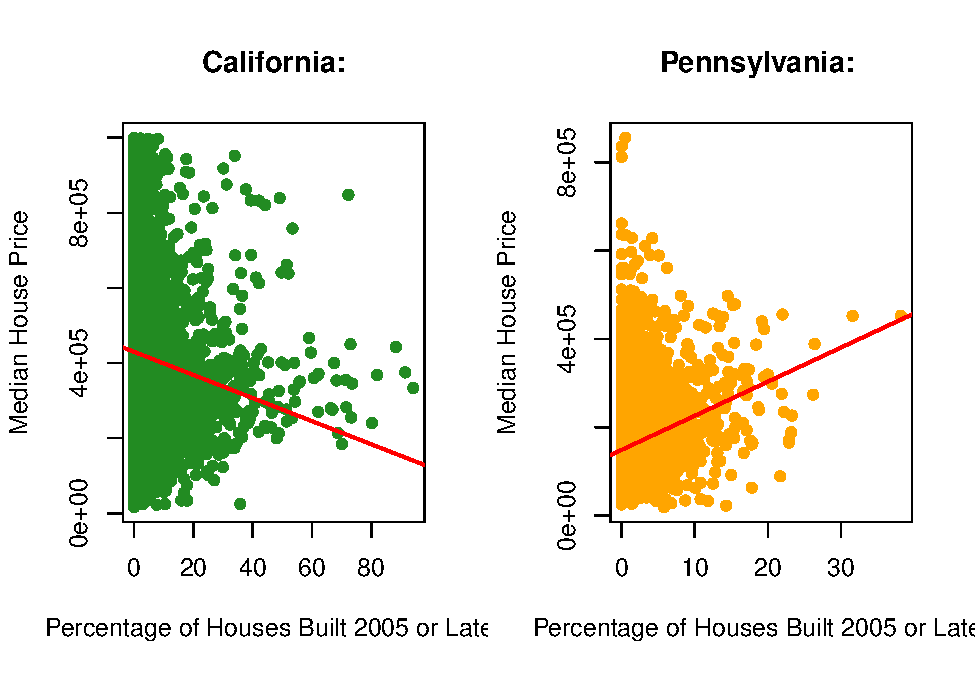
\includegraphics[keepaspectratio]{homework2_files/figure-latex/unnamed-chunk-8-1.pdf}}

\begin{Shaded}
\begin{Highlighting}[]
\FunctionTok{par}\NormalTok{(}\AttributeTok{mfrow =} \FunctionTok{c}\NormalTok{(}\DecValTok{1}\NormalTok{, }\DecValTok{1}\NormalTok{))  }
\end{Highlighting}
\end{Shaded}

\subsection{3 Nobody Home}\label{nobody-home}

\subsubsection{a}\label{a-1}

\begin{verbatim}
## 空置率最小值:  0
\end{verbatim}

\begin{verbatim}
## 空置率最大值:  0.965311
\end{verbatim}

\begin{verbatim}
## 空置率均值:  0.08888789
\end{verbatim}

\begin{verbatim}
## 空置率中位数:  0.06767283
\end{verbatim}

\subsubsection{b}\label{b-2}

\begin{Shaded}
\begin{Highlighting}[]
\FunctionTok{plot}\NormalTok{(}
  \AttributeTok{x =}\NormalTok{ ca\_pa\_clean}\SpecialCharTok{$}\NormalTok{vacancy\_rate, }
  \AttributeTok{y =}\NormalTok{ ca\_pa\_clean}\SpecialCharTok{$}\NormalTok{Median\_house\_value,}
  \AttributeTok{main =} \StringTok{"Vacancy Rate vs Median House Value"}\NormalTok{,}
  \AttributeTok{xlab =} \StringTok{"Vacancy Rate"}\NormalTok{,}
  \AttributeTok{ylab =} \StringTok{"Median House Value"}\NormalTok{,}
  \AttributeTok{pch =} \DecValTok{16}\NormalTok{,  }
  \AttributeTok{col =} \StringTok{"cornflowerblue"}  
\NormalTok{)}

\FunctionTok{abline}\NormalTok{(}\FunctionTok{lm}\NormalTok{(Median\_house\_value }\SpecialCharTok{\textasciitilde{}}\NormalTok{ vacancy\_rate, }\AttributeTok{data =}\NormalTok{ ca\_pa\_clean), }
       \AttributeTok{col =} \StringTok{"tomato"}\NormalTok{, }
       \AttributeTok{lwd =} \DecValTok{2}\NormalTok{)  }
\end{Highlighting}
\end{Shaded}

\pandocbounded{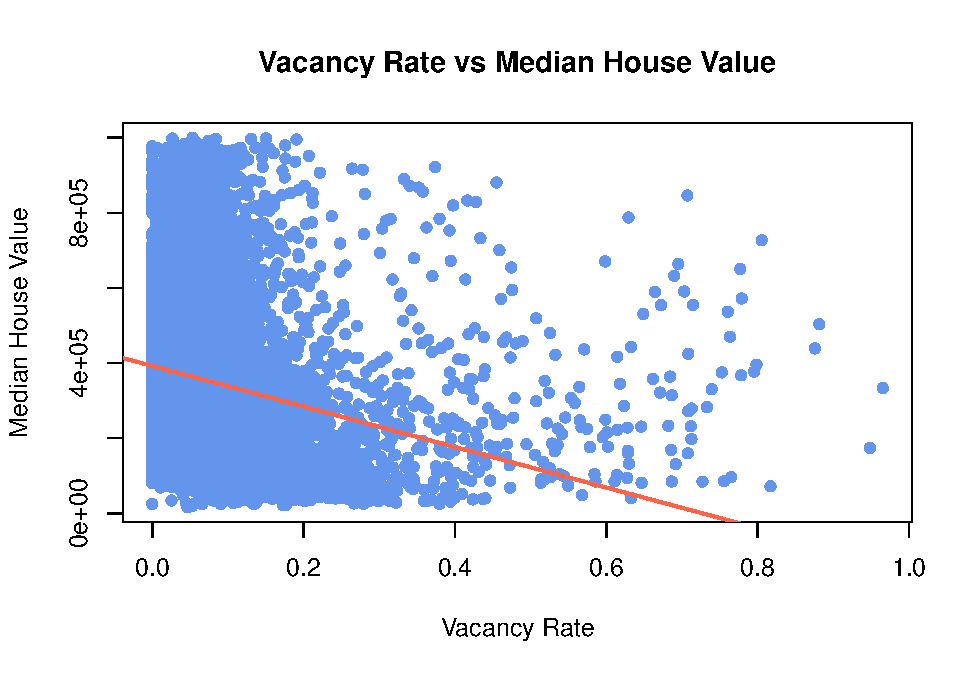
\includegraphics[keepaspectratio]{homework2_files/figure-latex/unnamed-chunk-10-1.pdf}}

\subsubsection{c}\label{c-1}

\begin{Shaded}
\begin{Highlighting}[]
\NormalTok{ca\_data }\OtherTok{\textless{}{-}}\NormalTok{ ca\_pa\_clean[ca\_pa\_clean}\SpecialCharTok{$}\NormalTok{STATEFP }\SpecialCharTok{==} \DecValTok{6}\NormalTok{, ]}
\NormalTok{pa\_data }\OtherTok{\textless{}{-}}\NormalTok{ ca\_pa\_clean[ca\_pa\_clean}\SpecialCharTok{$}\NormalTok{STATEFP }\SpecialCharTok{==} \DecValTok{42}\NormalTok{, ]}

\FunctionTok{par}\NormalTok{(}\AttributeTok{mfrow =} \FunctionTok{c}\NormalTok{(}\DecValTok{1}\NormalTok{, }\DecValTok{2}\NormalTok{))  }

\CommentTok{\# 加利福尼亚州散点图}
\FunctionTok{plot}\NormalTok{(}
  \AttributeTok{x =}\NormalTok{ ca\_data}\SpecialCharTok{$}\NormalTok{vacancy\_rate, }
  \AttributeTok{y =}\NormalTok{ ca\_data}\SpecialCharTok{$}\NormalTok{Median\_house\_value,}
  \AttributeTok{main =} \StringTok{"California: "}\NormalTok{,}
  \AttributeTok{xlab =} \StringTok{"Vacancy Rate"}\NormalTok{,}
  \AttributeTok{ylab =} \StringTok{"Median House Value"}\NormalTok{,}
  \AttributeTok{pch =} \DecValTok{16}\NormalTok{,}
  \AttributeTok{col =} \StringTok{"forestgreen"}
\NormalTok{)}
\FunctionTok{abline}\NormalTok{(}\FunctionTok{lm}\NormalTok{(Median\_house\_value }\SpecialCharTok{\textasciitilde{}}\NormalTok{ vacancy\_rate, }\AttributeTok{data =}\NormalTok{ ca\_data), }
       \AttributeTok{col =} \StringTok{"tomato"}\NormalTok{, }
       \AttributeTok{lwd =} \DecValTok{2}\NormalTok{)}

\CommentTok{\# 宾夕法尼亚州散点图}
\FunctionTok{plot}\NormalTok{(}
  \AttributeTok{x =}\NormalTok{ pa\_data}\SpecialCharTok{$}\NormalTok{vacancy\_rate, }
  \AttributeTok{y =}\NormalTok{ pa\_data}\SpecialCharTok{$}\NormalTok{Median\_house\_value,}
  \AttributeTok{main =} \StringTok{"Pennsylvania:"}\NormalTok{,}
  \AttributeTok{xlab =} \StringTok{"Vacancy Rate"}\NormalTok{,}
  \AttributeTok{ylab =} \StringTok{"Median House Value"}\NormalTok{,}
  \AttributeTok{pch =} \DecValTok{16}\NormalTok{,}
  \AttributeTok{col =} \StringTok{"orange"}
\NormalTok{)}
\FunctionTok{abline}\NormalTok{(}\FunctionTok{lm}\NormalTok{(Median\_house\_value }\SpecialCharTok{\textasciitilde{}}\NormalTok{ vacancy\_rate, }\AttributeTok{data =}\NormalTok{ pa\_data), }
       \AttributeTok{col =} \StringTok{"tomato"}\NormalTok{, }
       \AttributeTok{lwd =} \DecValTok{2}\NormalTok{)}
\end{Highlighting}
\end{Shaded}

\pandocbounded{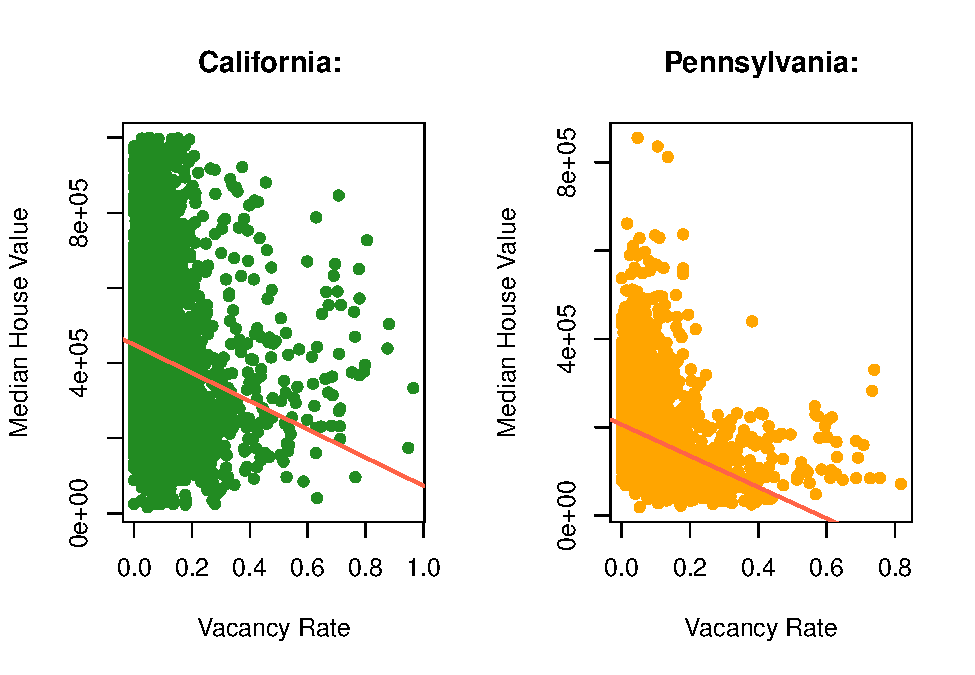
\includegraphics[keepaspectratio]{homework2_files/figure-latex/unnamed-chunk-11-1.pdf}}

\begin{Shaded}
\begin{Highlighting}[]
\FunctionTok{par}\NormalTok{(}\AttributeTok{mfrow =} \FunctionTok{c}\NormalTok{(}\DecValTok{1}\NormalTok{, }\DecValTok{1}\NormalTok{))  }
\end{Highlighting}
\end{Shaded}

两个州图像存在较大差异

\subsection{4}\label{section}

\subsubsection{a}\label{a-2}

\begin{Shaded}
\begin{Highlighting}[]
\NormalTok{ acca }\OtherTok{\textless{}{-}} \FunctionTok{c}\NormalTok{()}
 \ControlFlowTok{for}\NormalTok{ (tract }\ControlFlowTok{in} \DecValTok{1}\SpecialCharTok{:}\FunctionTok{nrow}\NormalTok{(ca\_pa\_clean)) \{}
 \ControlFlowTok{if}\NormalTok{ (ca\_pa\_clean}\SpecialCharTok{$}\NormalTok{STATEFP[tract] }\SpecialCharTok{==} \DecValTok{6}\NormalTok{) \{}
 \ControlFlowTok{if}\NormalTok{ (ca\_pa\_clean}\SpecialCharTok{$}\NormalTok{COUNTYFP[tract] }\SpecialCharTok{==} \DecValTok{1}\NormalTok{) \{}
\NormalTok{ acca }\OtherTok{\textless{}{-}} \FunctionTok{c}\NormalTok{(acca, tract)}
\NormalTok{ \}}
\NormalTok{ \}}
\NormalTok{ \}}
\NormalTok{ accamhv }\OtherTok{\textless{}{-}} \FunctionTok{c}\NormalTok{()}
 \ControlFlowTok{for}\NormalTok{ (tract }\ControlFlowTok{in}\NormalTok{ acca) \{}
\NormalTok{ accamhv }\OtherTok{\textless{}{-}} \FunctionTok{c}\NormalTok{(accamhv, ca\_pa\_clean[tract,}\DecValTok{10}\NormalTok{])}
\NormalTok{ \}}
 \FunctionTok{median}\NormalTok{(accamhv)}
\end{Highlighting}
\end{Shaded}

\begin{verbatim}
## [1] 474050
\end{verbatim}

遍历ca\_pa中每一行,将为加利福尼亚州Alameda
县的行索引加入到acca中(我这里ca\_pa\_clean是清理过的ca\_pa)

遍历 acca 中的行索引,提取这些行的第 10 列数据房价中位数,存储到
accanhv。然后取其中位数

\subsubsection{b}\label{b-3}

\begin{Shaded}
\begin{Highlighting}[]
\FunctionTok{median}\NormalTok{(ca\_pa\_clean[ca\_pa\_clean}\SpecialCharTok{$}\NormalTok{STATEFP }\SpecialCharTok{==} \DecValTok{6} \SpecialCharTok{\&}\NormalTok{ ca\_pa\_clean}\SpecialCharTok{$}\NormalTok{COUNTYFP }\SpecialCharTok{==} \DecValTok{1}\NormalTok{, }\DecValTok{10}\NormalTok{])}
\end{Highlighting}
\end{Shaded}

\begin{verbatim}
## [1] 474050
\end{verbatim}

\subsubsection{c}\label{c-2}

\begin{verbatim}
## Alameda 县平均新建住房比例: 2.820468
\end{verbatim}

\begin{verbatim}
## Santa Clara 县平均新建住房比例: 3.200319
\end{verbatim}

\begin{verbatim}
## Allegheny 县平均新建住房比例: 1.474219
\end{verbatim}

\subsubsection{d}\label{d-1}

\begin{verbatim}
## (i) 整个数据的相关性: -0.01893186
\end{verbatim}

\begin{verbatim}
## (ii) 加利福尼亚州的相关性: -0.1153604
\end{verbatim}

\begin{verbatim}
## (iii) 宾夕法尼亚州的相关性: 0.2681654
\end{verbatim}

\begin{verbatim}
## (iv) Alameda 县的相关性: 0.01303543
\end{verbatim}

\begin{verbatim}
## (v) Santa Clara 县的相关性: -0.1726203
\end{verbatim}

\begin{verbatim}
## (vi) Allegheny 县的相关性: 0.1939652
\end{verbatim}

\subsubsection{e.
绘制房价中位数与收入中位数的关系图(按县分组)}\label{e.-ux7ed8ux5236ux623fux4ef7ux4e2dux4f4dux6570ux4e0eux6536ux5165ux4e2dux4f4dux6570ux7684ux5173ux7cfbux56feux6309ux53bfux5206ux7ec4}

\begin{Shaded}
\begin{Highlighting}[]
\CommentTok{\# 加载 ggplot2 包(如果未加载)}
\FunctionTok{library}\NormalTok{(ggplot2)}

\NormalTok{alameda }\OtherTok{\textless{}{-}}\NormalTok{ ca\_pa\_clean[ca\_pa\_clean}\SpecialCharTok{$}\NormalTok{STATEFP }\SpecialCharTok{==} \DecValTok{6} \SpecialCharTok{\&}\NormalTok{ ca\_pa\_clean}\SpecialCharTok{$}\NormalTok{COUNTYFP }\SpecialCharTok{==} \DecValTok{1}\NormalTok{, ]}
\NormalTok{santa\_clara }\OtherTok{\textless{}{-}}\NormalTok{ ca\_pa\_clean[ca\_pa\_clean}\SpecialCharTok{$}\NormalTok{STATEFP }\SpecialCharTok{==} \DecValTok{6} \SpecialCharTok{\&}\NormalTok{ ca\_pa\_clean}\SpecialCharTok{$}\NormalTok{COUNTYFP }\SpecialCharTok{==} \DecValTok{85}\NormalTok{, ]}
\NormalTok{allegheny }\OtherTok{\textless{}{-}}\NormalTok{ ca\_pa\_clean[ca\_pa\_clean}\SpecialCharTok{$}\NormalTok{STATEFP }\SpecialCharTok{==} \DecValTok{42} \SpecialCharTok{\&}\NormalTok{ ca\_pa\_clean}\SpecialCharTok{$}\NormalTok{COUNTYFP }\SpecialCharTok{==} \DecValTok{3}\NormalTok{, ]}

\CommentTok{\# 为每个县数据添加标识列,再合并,让数据框直接包含要引用的列}
\NormalTok{alameda}\SpecialCharTok{$}\NormalTok{County }\OtherTok{\textless{}{-}} \StringTok{"Alameda"}
\NormalTok{santa\_clara}\SpecialCharTok{$}\NormalTok{County }\OtherTok{\textless{}{-}} \StringTok{"Santa Clara"}
\NormalTok{allegheny}\SpecialCharTok{$}\NormalTok{County }\OtherTok{\textless{}{-}} \StringTok{"Allegheny"}

\NormalTok{county\_data }\OtherTok{\textless{}{-}} \FunctionTok{rbind}\NormalTok{(alameda, santa\_clara, allegheny)}

\CommentTok{\# 使用 ggplot2 绘制分组散点图,直接引用列名}
\FunctionTok{ggplot}\NormalTok{(county\_data, }\FunctionTok{aes}\NormalTok{(}\AttributeTok{x =}\NormalTok{ Median\_household\_income, }\AttributeTok{y =}\NormalTok{ Median\_house\_value, }\AttributeTok{color =}\NormalTok{ County)) }\SpecialCharTok{+}
  \FunctionTok{geom\_point}\NormalTok{(}\AttributeTok{alpha =} \FloatTok{0.6}\NormalTok{, }\AttributeTok{size =} \DecValTok{2}\NormalTok{) }\SpecialCharTok{+}  
  \FunctionTok{geom\_smooth}\NormalTok{(}\AttributeTok{method =} \StringTok{"lm"}\NormalTok{, }\AttributeTok{se =} \ConstantTok{FALSE}\NormalTok{, }\AttributeTok{linetype =} \StringTok{"dashed"}\NormalTok{) }\SpecialCharTok{+}  
  \FunctionTok{labs}\NormalTok{(}
    \AttributeTok{title =} \StringTok{"房价中位数与收入中位数的关系)"}\NormalTok{,}
    \AttributeTok{x =} \StringTok{"收入中位数(美元)"}\NormalTok{,}
    \AttributeTok{y =} \StringTok{"房价中位数(美元)"}\NormalTok{,}
    \AttributeTok{color =} \StringTok{"县名"}
\NormalTok{  ) }\SpecialCharTok{+}
  \FunctionTok{theme\_minimal}\NormalTok{() }\SpecialCharTok{+}  
  \FunctionTok{theme}\NormalTok{(}
    \AttributeTok{plot.title =} \FunctionTok{element\_text}\NormalTok{(}\AttributeTok{hjust =} \FloatTok{0.5}\NormalTok{, }\AttributeTok{face =} \StringTok{"bold"}\NormalTok{), }
    \AttributeTok{legend.position =} \StringTok{"bottom"}\NormalTok{,  }
    \AttributeTok{axis.text =} \FunctionTok{element\_text}\NormalTok{(}\AttributeTok{size =} \DecValTok{10}\NormalTok{), }
    \AttributeTok{axis.title =} \FunctionTok{element\_text}\NormalTok{(}\AttributeTok{size =} \DecValTok{12}\NormalTok{, }\AttributeTok{face =} \StringTok{"bold"}\NormalTok{) }
\NormalTok{  ) }\SpecialCharTok{+}
  \FunctionTok{scale\_color\_manual}\NormalTok{(}\AttributeTok{values =} \FunctionTok{c}\NormalTok{(}
    \StringTok{"Alameda"} \OtherTok{=} \StringTok{"\#3366CC"}\NormalTok{,      }\CommentTok{\# 蓝色,区分 Alameda 县}
    \StringTok{"Santa Clara"} \OtherTok{=} \StringTok{"\#DC3912"}\NormalTok{,  }\CommentTok{\# 红色,区分 Santa Clara 县}
    \StringTok{"Allegheny"} \OtherTok{=} \StringTok{"\#FF9900"}    \CommentTok{\# 橙色,区分 Allegheny 县}
\NormalTok{  ))}
\end{Highlighting}
\end{Shaded}

\begin{verbatim}
## `geom_smooth()` using formula = 'y ~ x'
\end{verbatim}

\pandocbounded{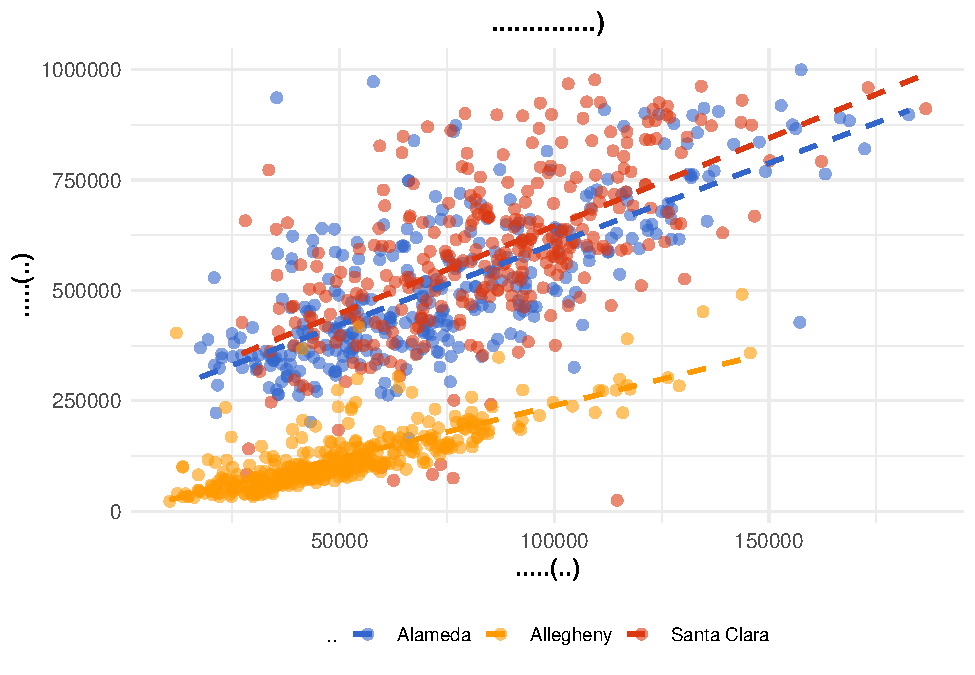
\includegraphics[keepaspectratio]{homework2_files/figure-latex/unnamed-chunk-16-1.pdf}}

\subsection{MB.Ch1}\label{mb.ch1}

\begin{Shaded}
\begin{Highlighting}[]
\NormalTok{gender}\OtherTok{\textless{}{-}} \FunctionTok{factor}\NormalTok{(}\FunctionTok{c}\NormalTok{(}\FunctionTok{rep}\NormalTok{(}\StringTok{"female"}\NormalTok{,}\DecValTok{91}\NormalTok{),}\FunctionTok{rep}\NormalTok{(}\StringTok{"male"}\NormalTok{,}\DecValTok{92}\NormalTok{)))}
\FunctionTok{table}\NormalTok{(gender)}
\end{Highlighting}
\end{Shaded}

\begin{verbatim}
## gender
## female   male 
##     91     92
\end{verbatim}

\begin{Shaded}
\begin{Highlighting}[]
\CommentTok{\#初始 gender 因子有 female(91 个)和 male(92 个),table 按默认水平统计,输出对应数量}
\end{Highlighting}
\end{Shaded}

\begin{Shaded}
\begin{Highlighting}[]
\NormalTok{gender }\OtherTok{\textless{}{-}} \FunctionTok{factor}\NormalTok{(gender, }\AttributeTok{levels=}\FunctionTok{c}\NormalTok{(}\StringTok{"male"}\NormalTok{, }\StringTok{"female"}\NormalTok{))}
 \FunctionTok{table}\NormalTok{(gender)}
\end{Highlighting}
\end{Shaded}

\begin{verbatim}
## gender
##   male female 
##     92     91
\end{verbatim}

\begin{Shaded}
\begin{Highlighting}[]
 \CommentTok{\# 重新指定因子水平,table 按新水平顺序(male 在前、female 在后)统计}
\end{Highlighting}
\end{Shaded}

\begin{Shaded}
\begin{Highlighting}[]
\NormalTok{ gender }\OtherTok{\textless{}{-}} \FunctionTok{factor}\NormalTok{(gender, }\AttributeTok{levels=}\FunctionTok{c}\NormalTok{(}\StringTok{"Male"}\NormalTok{, }\StringTok{"female"}\NormalTok{))}
 \FunctionTok{table}\NormalTok{(gender)}
\end{Highlighting}
\end{Shaded}

\begin{verbatim}
## gender
##   Male female 
##      0     91
\end{verbatim}

\begin{Shaded}
\begin{Highlighting}[]
 \CommentTok{\#指定水平为 c("Male", "female"),原数据无 Male 水平,仅 female 匹配,故 Male 计数为 0,female 为 91}
\end{Highlighting}
\end{Shaded}

\begin{Shaded}
\begin{Highlighting}[]
 \FunctionTok{table}\NormalTok{(gender, }\AttributeTok{exclude=}\ConstantTok{NULL}\NormalTok{)}
\end{Highlighting}
\end{Shaded}

\begin{verbatim}
## gender
##   Male female   <NA> 
##      0     91     92
\end{verbatim}

\begin{Shaded}
\begin{Highlighting}[]
\CommentTok{\# 加入exclude=NULL 后,未匹配的male被归为NA显示,输出 Male(0)、female(91)、\textless{}NA\textgreater{}}
\end{Highlighting}
\end{Shaded}

\subsection{MB.Ch1.2}\label{mb.ch1.2}

\subsubsection{a}\label{a-3}

\begin{Shaded}
\begin{Highlighting}[]
\NormalTok{prop\_exceed }\OtherTok{\textless{}{-}} \ControlFlowTok{function}\NormalTok{(x, cutoff) \{}
  \FunctionTok{mean}\NormalTok{(x }\SpecialCharTok{\textgreater{}}\NormalTok{ cutoff)}
\NormalTok{\}}
\NormalTok{x }\OtherTok{\textless{}{-}} \DecValTok{1}\SpecialCharTok{:}\DecValTok{100}
\CommentTok{\# 用 1到100计算超过50的比例}
\NormalTok{result\_a }\OtherTok{\textless{}{-}} \FunctionTok{prop\_exceed}\NormalTok{(x, }\DecValTok{50}\NormalTok{)}
\end{Highlighting}
\end{Shaded}

\subsubsection{b}\label{b-4}

\begin{Shaded}
\begin{Highlighting}[]
\NormalTok{prop\_exceed }\OtherTok{\textless{}{-}} \ControlFlowTok{function}\NormalTok{(x, cutoff) \{}
  \FunctionTok{mean}\NormalTok{(x }\SpecialCharTok{\textgreater{}}\NormalTok{ cutoff)}
\NormalTok{\}}

\FunctionTok{library}\NormalTok{(Devore7)}
\end{Highlighting}
\end{Shaded}

\begin{verbatim}
## Loading required package: MASS
\end{verbatim}

\begin{verbatim}
## Loading required package: lattice
\end{verbatim}

\begin{Shaded}
\begin{Highlighting}[]
\FunctionTok{data}\NormalTok{(}\StringTok{"ex01.36"}\NormalTok{)}

\CommentTok{\# 将秒换算为分钟}
\NormalTok{escape\_times }\OtherTok{\textless{}{-}}\NormalTok{ ex01}\FloatTok{.36}\SpecialCharTok{$}\NormalTok{C1 }\SpecialCharTok{/} \DecValTok{60}  

\FunctionTok{dotplot}\NormalTok{(escape\_times, }
        \AttributeTok{main =} \StringTok{"Distribution of Escape Times (in minutes)"}\NormalTok{, }
        \AttributeTok{xlab =} \StringTok{"Escape Time (minutes)"}\NormalTok{)}
\end{Highlighting}
\end{Shaded}

\pandocbounded{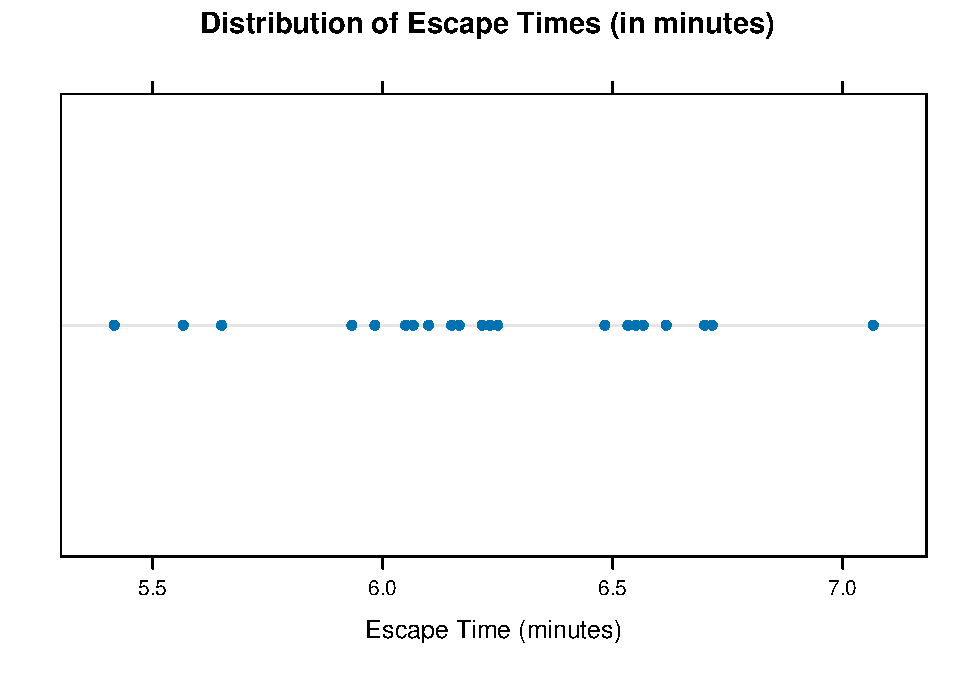
\includegraphics[keepaspectratio]{homework2_files/figure-latex/unnamed-chunk-22-1.pdf}}

\begin{Shaded}
\begin{Highlighting}[]
\CommentTok{\# 计算超过 7 分钟的比例}
\NormalTok{result\_b }\OtherTok{\textless{}{-}} \FunctionTok{prop\_exceed}\NormalTok{(escape\_times, }\DecValTok{7}\NormalTok{)}
\NormalTok{result\_b}
\end{Highlighting}
\end{Shaded}

\begin{verbatim}
## [1] 0.03846154
\end{verbatim}

\subsection{MB.Ch 1.18}\label{mb.ch-1.18}

\begin{Shaded}
\begin{Highlighting}[]
\FunctionTok{library}\NormalTok{(MASS)}
\FunctionTok{data}\NormalTok{(Rabbit)}


\NormalTok{rabbit\_unstacked }\OtherTok{\textless{}{-}} \FunctionTok{unstack}\NormalTok{(Rabbit, BPchange }\SpecialCharTok{\textasciitilde{}}\NormalTok{ Animal)}


\NormalTok{Rabbit}\SpecialCharTok{$}\NormalTok{id }\OtherTok{\textless{}{-}} \FunctionTok{with}\NormalTok{(Rabbit, }\FunctionTok{paste}\NormalTok{(Dose, Treatment, }\AttributeTok{sep =} \StringTok{"\_"}\NormalTok{))}

\NormalTok{dose\_treatment }\OtherTok{\textless{}{-}} \FunctionTok{unique}\NormalTok{(Rabbit[}\FunctionTok{c}\NormalTok{(}\StringTok{"Dose"}\NormalTok{, }\StringTok{"Treatment"}\NormalTok{, }\StringTok{"id"}\NormalTok{)])}


\NormalTok{final\_result }\OtherTok{\textless{}{-}} \FunctionTok{cbind}\NormalTok{(dose\_treatment, rabbit\_unstacked)}


\NormalTok{final\_result}\SpecialCharTok{$}\NormalTok{id }\OtherTok{\textless{}{-}} \ConstantTok{NULL}


\NormalTok{final\_result }\OtherTok{\textless{}{-}}\NormalTok{ final\_result[, }\FunctionTok{c}\NormalTok{(}\StringTok{"Treatment"}\NormalTok{, }\StringTok{"Dose"}\NormalTok{, }\StringTok{"R1"}\NormalTok{, }\StringTok{"R2"}\NormalTok{, }\StringTok{"R3"}\NormalTok{, }\StringTok{"R4"}\NormalTok{, }\StringTok{"R5"}\NormalTok{)]}

\NormalTok{final\_result }\OtherTok{\textless{}{-}}\NormalTok{ final\_result[}\FunctionTok{order}\NormalTok{(final\_result}\SpecialCharTok{$}\NormalTok{Dose), ]}

\FunctionTok{rownames}\NormalTok{(final\_result) }\OtherTok{\textless{}{-}} \ConstantTok{NULL}

\NormalTok{final\_result}
\end{Highlighting}
\end{Shaded}

\begin{verbatim}
##    Treatment   Dose    R1    R2    R3    R4   R5
## 1    Control   6.25  0.50  1.00  0.75  1.25  1.5
## 2        MDL   6.25  1.25  1.40  0.75  2.60  2.4
## 3    Control  12.50  4.50  1.25  3.00  1.50  1.5
## 4        MDL  12.50  0.75  1.70  2.30  1.20  2.5
## 5    Control  25.00 10.00  4.00  3.00  6.00  5.0
## 6        MDL  25.00  4.00  1.00  3.00  2.00  1.5
## 7    Control  50.00 26.00 12.00 14.00 19.00 16.0
## 8        MDL  50.00  9.00  2.00  5.00  3.00  2.0
## 9    Control 100.00 37.00 27.00 22.00 33.00 20.0
## 10       MDL 100.00 25.00 15.00 26.00 11.00  9.0
## 11   Control 200.00 32.00 29.00 24.00 33.00 18.0
## 12       MDL 200.00 37.00 28.00 25.00 22.00 19.0
\end{verbatim}

\end{document}
